%!TeX root=../pridetop.tex
\chapter[Chapter \thechapter]{}
	
	
\begin{figure}[t!]
\centering
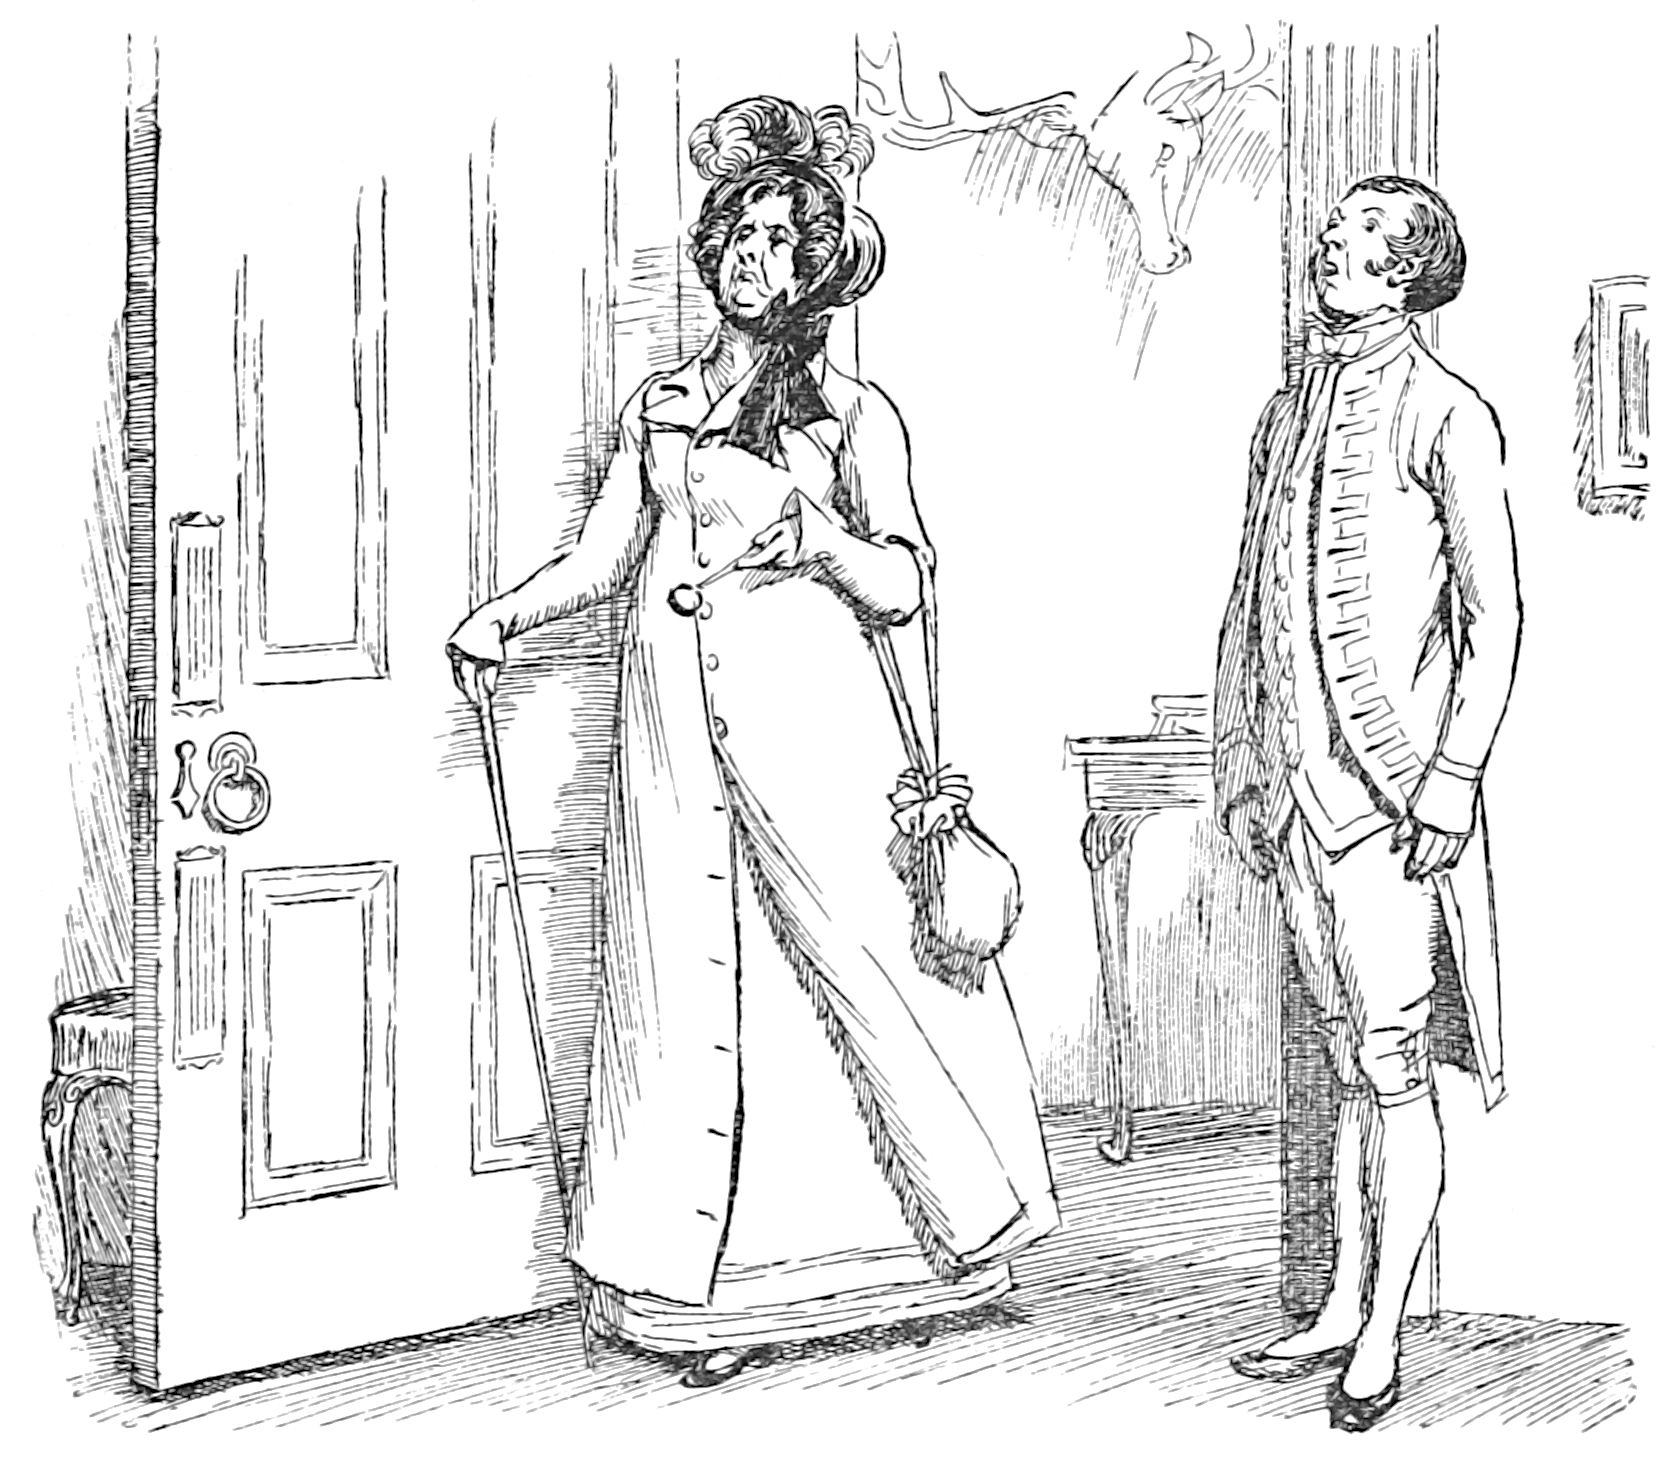
\includegraphics[width=\linewidth]{56top}
\captionlistentry{Headpiece to Chapter \thechapter}
\end{figure}


\lettrine[lines=6,image=true]{initials/chap56o}{ne}  morning, about a week after Bingley's engagement with Jane had been formed, as he and the females of the family were sitting together in the dining-room, their attention was suddenly drawn to the window by the sound of a carriage; and they perceived a chaise and four driving up the lawn. It was too early in the morning for visitors; and besides, the equipage did not answer to that of any of their neighbours. The horses were post; and neither the carriage, nor the livery of the servant who preceded it, were familiar to them. As it was certain, however, that somebody was coming, Bingley instantly prevailed on Miss Bennet to avoid the confinement of such an intrusion, and walk away with him into the shrubbery. They both set off; and the conjectures of the remaining three continued, though with little satisfaction, till the door was thrown open, and their visitor entered. It was Lady Catherine de Bourgh.

They were of course all intending to be surprised: but their astonishment was beyond their expectation; and on the part of Mrs Bennet and Kitty, though she was perfectly unknown to them, even inferior to what Elizabeth felt.

She entered the room with an air more than usually ungracious, made no other reply to Elizabeth's salutation than a slight inclination of the head, and sat down without saying a word. Elizabeth had mentioned her name to her mother on her Ladyship's entrance, though no request of introduction had been made.

Mrs Bennet, all amazement, though flattered by having a guest of such high importance, received her with the utmost politeness. After sitting for a moment in silence, she said, very stiffly, to Elizabeth,—

<I hope you are well, Miss Bennet. That lady, I suppose, is your mother?>

Elizabeth replied very concisely that she was.

<And \textit{that}, I suppose, is one of your sisters?>

<Yes, madam,> said Mrs Bennet, delighted to speak to a Lady Catherine. <She is my youngest girl but one. My youngest of all is lately married, and my eldest is somewhere about the ground, walking with a young man, who, I believe, will soon become a part of the family.>

<You have a very small park here,> returned Lady Catherine, after a short silence.

<It is nothing in comparison of Rosings, my Lady, I dare say; but, I assure you, it is much larger than Sir William Lucas's.>

<This must be a most inconvenient sitting-room for the evening in summer: the windows are full west.>

Mrs Bennet assured her that they never sat there after dinner; and then added,—

<May I take the liberty of asking your Ladyship whether you left Mr and Mrs Collins well?>

<Yes, very well. I saw them the night before last.>

Elizabeth now expected that she would produce a letter for her from Charlotte, as it seemed the only probable motive for her calling. But no letter appeared, and she was completely puzzled.

Mrs Bennet, with great civility, begged her Ladyship to take some refreshment: but Lady Catherine very resolutely, and not very politely, declined eating anything; and then, rising up, said to Elizabeth,—

<Miss Bennet, there seemed to be a prettyish kind of a little wilderness on one side of your lawn. I should be glad to take a turn in it, if you will favour me with your company.>

<Go, my dear,> cried her mother, <and show her Ladyship about the different walks. I think she will be pleased with the hermitage.>

Elizabeth obeyed; and, running into her own room for her parasol, attended her noble guest downstairs. As they passed through the hall, Lady Catherine opened the doors into the dining-parlour and drawing-room, and pronouncing them, after a short survey, to be decent-looking rooms, walked on.

Her carriage remained at the door, and Elizabeth saw that her waiting-woman was in it. They proceeded in silence along the gravel walk that led to the copse; Elizabeth was determined to make no effort for conversation with a woman who was now more than usually insolent and disagreeable.

<How could I ever think her like her nephew?> said she, as she looked in her face.

As soon as they entered the copse, Lady Catherine began in the following manner:—

<You can be at no loss, Miss Bennet, to understand the reason of my journey hither. Your own heart, your own conscience, must tell you why I come.>

Elizabeth looked with unaffected astonishment.

<Indeed, you are mistaken, madam; I have not been at all able to account for the honour of seeing you here.>

<Miss Bennet,> replied her Ladyship, in an angry tone, <you ought to know that I am not to be trifled with. But however insincere \textit{you} may choose to be, you shall not find \textit{me} so. My character has ever been celebrated for its sincerity and frankness; and in a cause of such moment as this, I shall certainly not depart from it. A report of a most alarming nature reached me two days ago. I was told, that not only your sister was on the point of being most advantageously married, but that \textit{you}—that Miss Elizabeth Bennet would, in all likelihood, be soon afterwards united to my nephew—my own nephew, Mr Darcy. Though I \textit{know} it must be a scandalous falsehood, though I would not injure him so much as to suppose the truth of it possible, I instantly resolved on setting off for this place, that I might make my sentiments known to you.>

<If you believed it impossible to be true,> said Elizabeth, colouring with astonishment and disdain, <I wonder you took the trouble of coming so far. What could your Ladyship propose by it?>

<At once to insist upon having such a report universally contradicted.>

<Your coming to Longbourn, to see me and my family,> said Elizabeth coolly, <will be rather a confirmation of it—if, indeed, such a report is in existence.>

<If! do you then pretend to be ignorant of it? Has it not been industriously circulated by yourselves? Do you not know that such a report is spread abroad?>

<I never heard that it was.>

<And can you likewise declare, that there is no \textit{foundation} for it?>

<I do not pretend to possess equal frankness with your Ladyship. \textit{You} may ask questions which \textit{I} shall not choose to answer.>

<This is not to be borne. Miss Bennet, I insist on being satisfied. Has he, has my nephew, made you an offer of marriage?>

<Your Ladyship has declared it to be impossible.>

<It ought to be so; it must be so, while he retains the use of his reason. But \textit{your} arts and allurements may, in a moment of infatuation, have made him forget what he owes to himself and to all his family. You may have drawn him in.>

<If I have, I shall be the last person to confess it.>

<Miss Bennet, do you know who I am? I have not been accustomed to such language as this. I am almost the nearest relation he has in the world, and am entitled to know all his dearest concerns.>

<But you are not entitled to know \textit{mine}; nor will such behaviour as this ever induce me to be explicit.>

<Let me be rightly understood. This match, to which you have the presumption to aspire, can never take place. No, never. Mr Darcy is engaged to \textit{my daughter}. Now, what have you to say?>

<Only this,—that if he is so, you can have no reason to suppose he will make an offer to me.>

Lady Catherine hesitated for a moment, and then replied,—

<The engagement between them is of a peculiar kind. From their infancy, they have been intended for each other. It was the favourite wish of \textit{his} mother, as well as of hers. While in their cradles we planned the union; and now, at the moment when the wishes of both sisters would be accomplished, is their marriage to be prevented by a young woman of inferior birth, of no importance in the world, and wholly unallied to the family? Do you pay no regard to the wishes of his friends—to his tacit engagement with Miss de Bourgh? Are you lost to every feeling of propriety and delicacy? Have you not heard me say, that from his earliest hours he was destined for his cousin?>

<Yes; and I had heard it before. But what is that to me? If there is no other objection to my marrying your nephew, I shall certainly not be kept from it by knowing that his mother and aunt wished him to marry Miss de Bourgh. You both did as much as you could in planning the marriage. Its completion depended on others. If Mr Darcy is neither by honour nor inclination confined to his cousin, why is not he to make another choice? And if I am that choice, why may not I accept him?>

<Because honour, decorum, prudence—nay, interest—forbid it. Yes, Miss Bennet, interest; for do not expect to be noticed by his family or friends, if you wilfully act against the inclinations of all. You will be censured, slighted, and despised, by everyone connected with him. Your alliance will be a disgrace; your name will never even be mentioned by any of us.>

<These are heavy misfortunes,> replied Elizabeth. <But the wife of Mr Darcy must have such extraordinary sources of happiness necessarily attached to her situation, that she could, upon the whole, have no cause to repine.>

<Obstinate, headstrong girl! I am ashamed of you! Is this your gratitude for my attentions to you last spring? Is nothing due to me on that score? Let us sit down. You are to understand, Miss Bennet, that I came here with the determined resolution of carrying my purpose; nor will I be dissuaded from it. I have not been used to submit to any person's whims. I have not been in the habit of brooking disappointment.>

<\textit{That} will make your Ladyship's situation at present more pitiable; but it will have no effect on \textit{me}.>

<I will not be interrupted! Hear me in silence. My daughter and my nephew are formed for each other. They are descended, on the maternal side, from the same noble line; and, on the father's, from respectable, honourable, and ancient, though untitled, families. Their fortune on both sides is splendid. They are destined for each other by the voice of every member of their respective houses; and what is to divide them?—the upstart pretensions of a young woman without family, connections, or fortune! Is this to be endured? But it must not, shall not be! If you were sensible of your own good, you would not wish to quit the sphere in which you have been brought up.>

<In marrying your nephew, I should not consider myself as quitting that sphere. He is a gentleman; I am a gentleman's daughter; so far we are equal.>

<True. You \textit{are} a gentleman's daughter. But what was your mother? Who are your uncles and aunts? Do not imagine me ignorant of their condition.>

<Whatever my connections may be,> said Elizabeth, <if your nephew does not object to them, they can be nothing to \textit{you}.>

<Tell me, once for all, are you engaged to him?>

Though Elizabeth would not, for the mere purpose of obliging Lady Catherine, have answered this question, she could not but say, after a moment's deliberation,—

<I am not.>

Lady Catherine seemed pleased.

<And will you promise me never to enter into such an engagement?>

<I will make no promise of the kind.>

<Miss Bennet, I am shocked and astonished. I expected to find a more reasonable young woman. But do not deceive yourself into a belief that I will ever recede. I shall not go away till you have given me the assurance I require.>

<And I certainly \textit{never} shall give it. I am not to be intimidated into anything so wholly unreasonable. Your Ladyship wants Mr Darcy to marry your daughter; but would my giving you the wished-for promise make \textit{their} marriage at all more probable? Supposing him to be attached to me, would \textit{my} refusing to accept his hand make him wish to bestow it on his cousin? Allow me to say, Lady Catherine, that the arguments with which you have supported this extraordinary application have been as frivolous as the application was ill-judged. You have widely mistaken my character, if you think I can be worked on by such persuasions as these. How far your nephew might approve of your interference in \textit{his} affairs, I cannot tell; but you have certainly no right to concern yourself in mine. I must beg, therefore, to be importuned no further on the subject.>

<Not so hasty, if you please. I have by no means done. To all the objections I have already urged I have still another to add. I am no stranger to the particulars of your youngest sister's infamous elopement. I know it all; that the young man's marrying her was a patched-up business, at the expense of your father and uncle. And is \textit{such} a girl to be my nephew's sister? Is \textit{her} husband, who is the son of his late father's steward, to be his brother? Heaven and earth!—of what are you thinking? Are the shades of Pemberley to be thus polluted?>

<You can \textit{now} have nothing further to say,> she resentfully answered. <You have insulted me, in every possible method. I must beg to return to the house.>

And she rose as she spoke. Lady Catherine rose also, and they turned back. Her Ladyship was highly incensed.

<You have no regard, then, for the honour and credit of my nephew! Unfeeling, selfish girl! Do you not consider that a connection with you must disgrace him in the eyes of everybody?>

<Lady Catherine, I have nothing further to say. You know my sentiments.>

<You are then resolved to have him?>

<I have said no such thing. I am only resolved to act in that manner, which will, in my own opinion, constitute my happiness, without reference to \textit{you}, or to any person so wholly unconnected with me.>

<It is well. You refuse, then, to oblige me. You refuse to obey the claims of duty, honour, and gratitude. You are determined to ruin him in the opinion of all his friends, and make him the contempt of the world.>

<Neither duty, nor honour, nor gratitude,> replied Elizabeth, <has any possible claim on me, in the present instance. No principle of either would be violated by my marriage with Mr Darcy. And with regard to the resentment of his family, or the indignation of the world, if the former \textit{were} excited by his marrying me, it would not give me one moment's concern—and the world in general would have too much sense to join in the scorn.>

<And this is your real opinion! This is your final resolve! Very well. I shall now know how to act. Do not imagine, Miss Bennet, that your ambition will ever be gratified. I came to try you. I hoped to find you reasonable; but depend upon it I will carry my point.>

In this manner Lady Catherine talked on till they were at the door of the carriage, when, turning hastily round, she added,—

<I take no leave of you, Miss Bennet. I send no compliments to your mother. You deserve no such attention. I am most seriously displeased.>

Elizabeth made no answer; and without attempting to persuade her Ladyship to return into the house, walked quietly into it herself. She heard the carriage drive away as she proceeded upstairs. Her mother impatiently met her at the door of her dressing-room, to ask why Lady Catherine would not come in again and rest herself.

<She did not choose it,> said her daughter; <she would go.>

<She is a very fine-looking woman! and her calling here was prodigiously civil! for she only came, I suppose, to tell us the Collinses were well. She is on her road somewhere, I dare say; and so, passing through Meryton, thought she might as well call on you. I suppose she had nothing particular to say to you, Lizzy?>

Elizabeth was forced to give in to a little falsehood here; for to acknowledge the substance of their conversation was impossible.